\chapter{电化学电池与电解}\label{ch:g12:cells-and-electrolysis}

一部手机在冬季傍晚显示电量仅 1 \%，随即没电关机。插上电源过夜后，它
清晨便重新充满。电池内部，同一化学反应
白天沿一个方向进行并放出电能，夜间则
由充电器驱动，沿相反方向进行。氧化还原反应可以
在电子被导入导线时成为电能的来源；
而电流通过溶液时，可以促使一个
本不会自发进行的氧化还原反应发生。

\begin{recall}
氧化剂得电子，还原剂失电子；半反应式、
氧化还原电对与氧化还原反应（见\cref{ch:g11:redox}）。体系演化直至
$Q = K$（见\cref{ch:g12:equilibrium}）。含离子的溶液能导电
（见\cref{ch:g9:ions}）；摩尔与阿伏伽德罗常数
（见\cref{ch:g10:the-mole}）。
\end{recall}

\begin{omfigure}
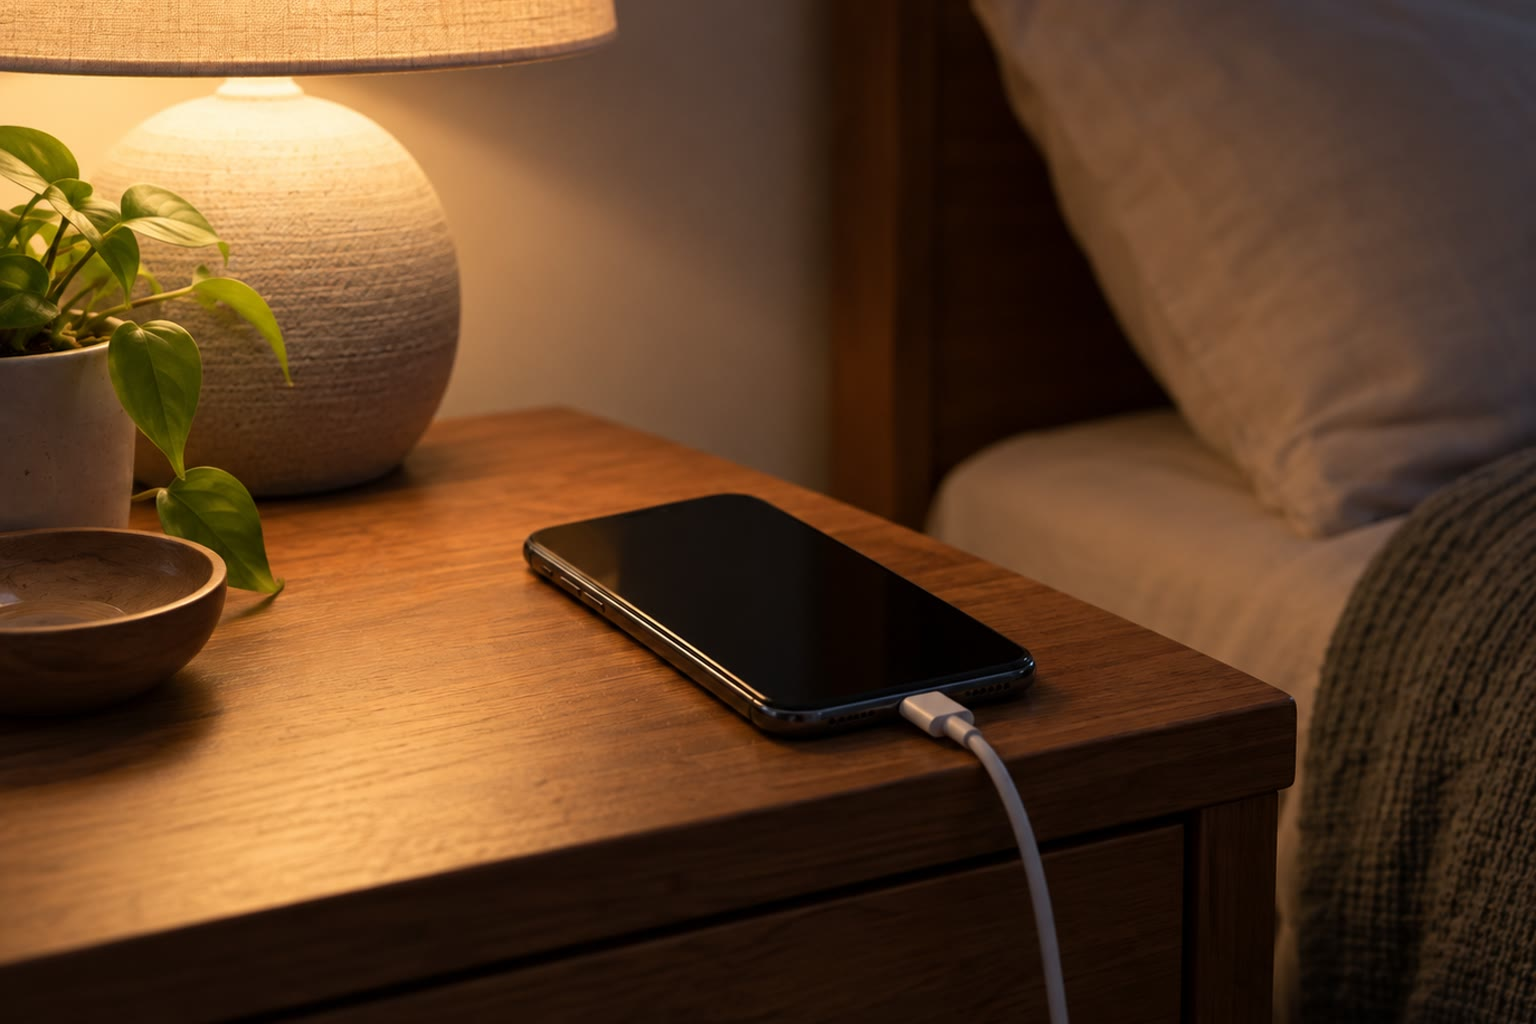
\includegraphics[width=0.45\linewidth]{images/book1/ai/g12-phone-charging.jpg}

{\small 给手机充电：一个反应在夜间被逆向驱动。}
\end{omfigure}

\section{将氧化还原反应一分为二}

将锌片浸入硫酸铜溶液中时，锌被氧化，
铜离子在锌片表面被还原，
\ce{Zn + Cu^{2+} -> Zn^{2+} + Cu}：电子直接由金属
转移至离子，能量以少量热量的形式散失。
将两个半电池分开，并用导线相连：电子现在必须
经导线传递，途中还可以点亮一盏灯。

\begin{definition}[电化学电池、半电池、盐桥]\label{def:g12:cells-and-electrolysis:cell}
\emph{电化学电池}\index{电化学电池}是利用
氧化还原反应产生电能的装置，其中氧化与还原
分别在两个彼此分隔的部分中进行。每一部分，
即浸于其离子溶液中的金属电极，是一个
\emph{半电池}\index{半电池}。\emph{盐桥}\index{盐桥}，
即浸有离子溶液的管子或纸条，连接两个
溶液并使电路闭合，同时使二者保持分隔。
\end{definition}

\begin{definition}[阳极、阴极]\label{def:g12:cells-and-electrolysis:anode}
发生氧化反应的电极称为
\emph{阳极}\index{阳极}；发生还原反应的电极
称为\emph{阴极}\index{阴极}。
\end{definition}

\begin{omfigure}
\begin{tikzpicture}[font=\small, scale=1.25]
  \pic[transform shape] at (0,0) {beaker={0.7}{black!6}};
  \pic[transform shape] at (4,0) {beaker={0.7}{cyan!70!blue!35}};
  \pic[transform shape] (zn) at (-0.3,0.25) {electrode={black!30}};
  \pic[transform shape] (cu) at (4.3,0.25) {electrode={orange!70!brown}};
  \pic[transform shape] at (0.35,0.6) {saltbridge={3.3}};
  \pic[transform shape] (v) at (2,3.9) {meter={1.10 V}};
  \draw[black!70, thick] (zn-top) |- (1.0,3.4) -| (v-a);
  \draw[black!70, thick] (cu-top) |- (3.0,3.4) -| (v-b);
  \draw[->, omProp, very thick] (0.2,3.55) -- (1.0,3.55);
  \draw[->, omProp, very thick] (3.0,3.55) -- (3.8,3.55);
  \node[omProp, font=\footnotesize] at (0.6,3.75) {$e^-$};
  \node[omProp, font=\footnotesize] at (3.4,3.75) {$e^-$};
  \node[anchor=north, align=center] at (-0.2,-0.15) {阳极 ($-$)：锌 \\ \ce{Zn -> Zn^{2+} + 2e-}};
  \node[anchor=north, align=center] at (4.2,-0.15) {阴极 ($+$)：铜 \\ \ce{Cu^{2+} + 2e- -> Cu}};
  \node[font=\footnotesize, anchor=east, align=right] at (-0.95,0.7) {\ce{Zn^{2+}}\\ \ce{SO4^{2-}}};
  \node[font=\footnotesize, anchor=west, align=left] at (4.95,0.7) {\ce{Cu^{2+}}\\ \ce{SO4^{2-}}};
  \node[font=\footnotesize, align=center] at (2,2.45) {盐桥 \\ (\ce{K+}, \ce{NO3-})};
\end{tikzpicture}

{\small 丹尼尔电池。电子经导线离开锌阳极，
进入铜阴极；在盐桥中，离子移动以保持
各溶液呈电中性。}
\end{omfigure}

\begin{proposition}[电子的流向]\label{prop:g12:cells-and-electrolysis:flow}
在输出电流的电池中，电子由阳极离开电池，
在阳极处因氧化反应而产生，经外电路传输，
由阴极进入电池，在阴极处被还原反应
消耗。阳极为负接线柱，阴极为正
接线柱。电池内部，电流由离子承载：阳离子
向阴极移动，阴离子向阳极移动。
\end{proposition}

\begin{proof}
氧化反应在阳极产生电子，还原反应在
阴极消耗电子；导线是两者之间唯一的通路。若无
盐桥，每种溶液都会带电，而盐桥中的离子
可防止这一情况。
\end{proof}

\begin{method}[描述一个电池]\label{met:g12:cells-and-electrolysis:describe}
\begin{enumerate}
  \item 写出自发进行的总氧化还原反应。
  \item 将其拆分为两个半反应式：氧化反应（阳极）与
        还原反应（阴极）。
  \item 标出极性：阳极 $-$，阴极 $+$；导线中电子的方向
        （由阳极到阴极）以及电流的方向
        （由阴极到阳极）。
  \item 描述盐桥中离子的运动。
\end{enumerate}
\end{method}


\begin{history}[伏打电堆，1800 年]
1800 年，物理学家亚历山德罗·伏打把两种不同的金属圆片叠放在一起，
即锌与铜或银，中间以浸过
盐水的布片隔开，获得了稳定的电流：这就是第一个电池。它
为物理学家提供了第一个连续的电源，并
为化学家提供了一种新工具：短短几年内，电解便首次分离出钠
和钾。
\end{history}

\begin{omfigure}
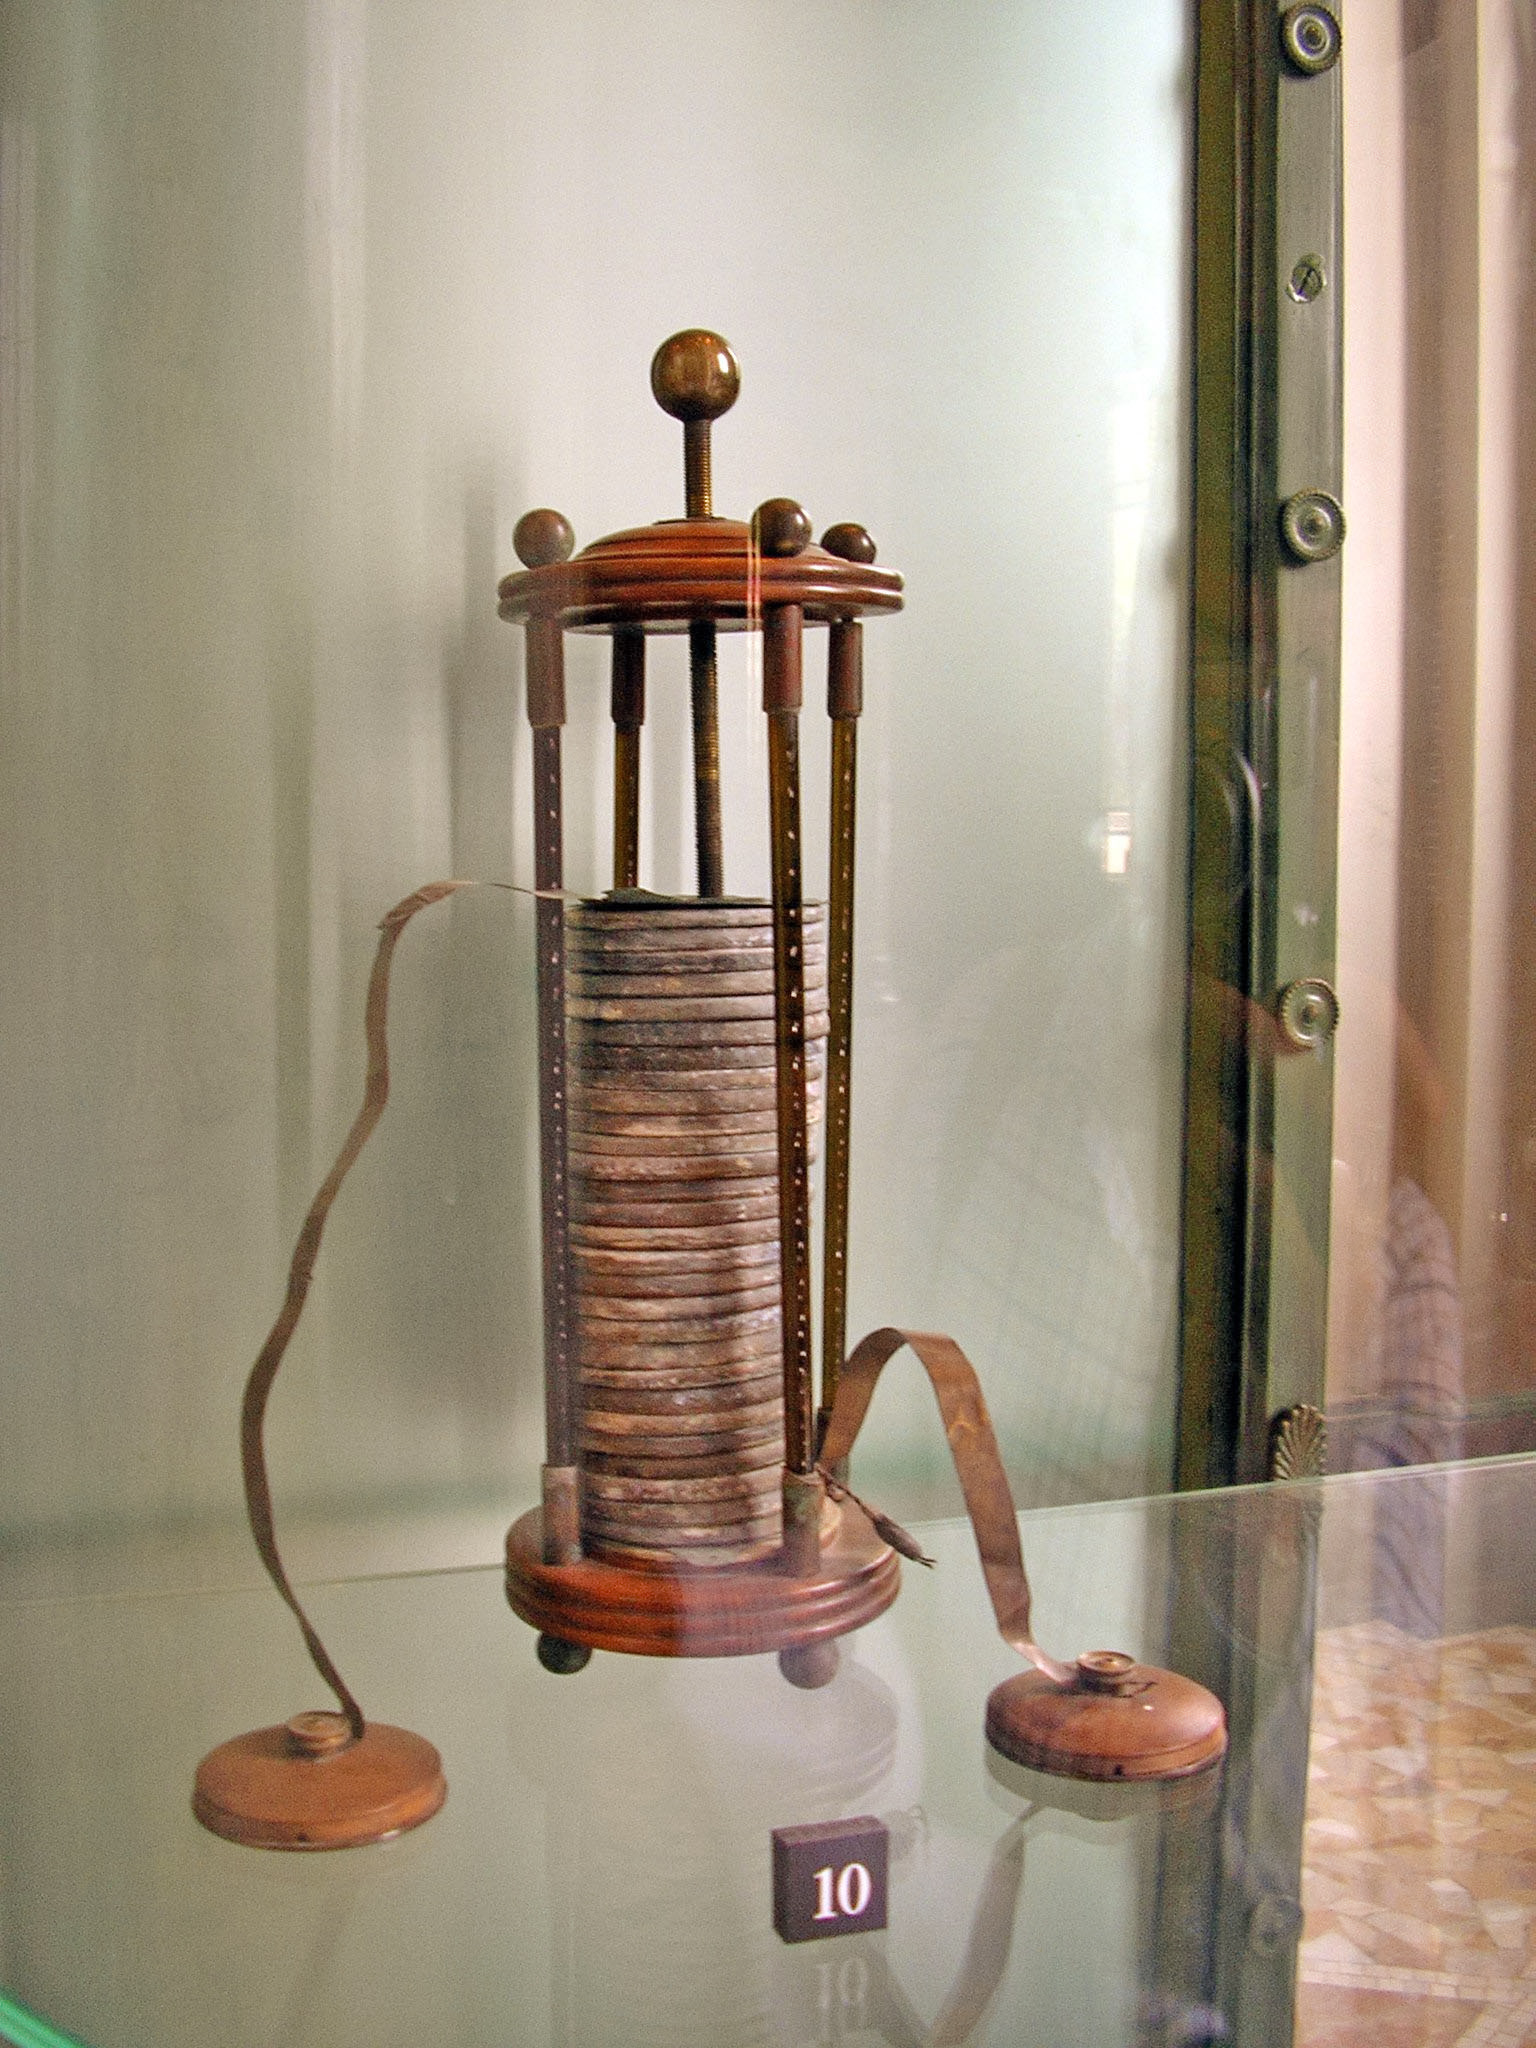
\includegraphics[width=0.24\linewidth]{images/book1/volta-pile.jpg}

{\small 博物馆中的伏打电堆。照片：GuidoB，CC BY-SA 3.0。}
\end{omfigure}

\section{电池的电压}

\begin{definition}[电池电压]\label{def:g12:cells-and-electrolysis:emf}
\emph{电池电压}\index{电池电压}是指在电池不输出电流（断开的电路）时，
用电压表测得的电池两接线柱之间的电压；
当电压表的正接线柱接在
阴极上时，该电压为正。
\end{definition}

\begin{example}[丹尼尔电池]\label{ex:g12:cells-and-electrolysis:daniell}
% ledger: e0:Cu, e0:Zn, emf:Daniell
两种溶液浓度均为\qty{1}{mol/L}时，丹尼尔电池
的电压为\qty{1.10}{V}。由电极电势表预测此类电压的方法，
详见本科一年级分册。
\end{example}

\begin{remark}[电池为何会耗尽]\label{rem:g12:cells-and-electrolysis:runs-down}
电池的反应\ce{Zn + Cu^{2+} -> Zn^{2+} + Cu}的平衡常数 $K$ 很大。
电池工作时，$Q = [\ce{Zn^{2+}}]/[\ce{Cu^{2+}}]$
增大，只要 $Q < K$，反应就会持续进行。当
某一反应物耗尽（锌或铜离子）时，电流停止，
电池即“没电”。
\end{remark}

\section{电荷与电量}

\begin{definition}[法拉第常数，电量]\label{def:g12:cells-and-electrolysis:capacity}
\emph{法拉第常数}\index{法拉第常数} $F$ 为一摩尔电子所带的
电荷量，$F = N_A e = \qty{96485}{C/mol}$。
\emph{电量}\index{电量}是指电池所能输出的
最大电荷量，通常以安时表示：$\qty{1}{A.h} = \qty{3600}{C}$。
\end{definition}

\begin{proposition}[电荷与电子的物质的量]\label{prop:g12:cells-and-electrolysis:charge}
% ledger: const:F, const:NA, const:e
电流 $I$ 在时间 $\Delta t$ 内通过时，携带的电荷量为
$Q = I\,\Delta t$，即电子的物质的量为
\[
  n(e^-) = \frac{Q}{F} = \frac{I\,\Delta t}{F} .
\]
\end{proposition}

\begin{proof}
每个电子带有元电荷 $e$，$n$ 摩尔电子
所带的电荷为 $n N_A e = n F$。
\end{proof}

\begin{example}[丹尼尔电池的电量]\label{ex:g12:cells-and-electrolysis:capacity}
% ledger: aw:Zn, const:F
锌电极中可参与反应的锌为\qty{6.5}{g}，即
$6.5/65.4 = \qty{0.099}{mol}$。每个锌原子给出两个电子：
因此 $n(e^-) = \qty{0.199}{mol}$，$Q = 0.199 \times 96485 = \qty{1.9e4}{C}$，
约合 $\qty{1.9e4}{}/3600 = \qty{5.3}{A.h}$，
前提是铜离子不会先耗尽。
\end{example}

\section{电解}

\begin{definition}[电解，蓄电池]\label{def:g12:cells-and-electrolysis:electrolysis}
\emph{电解}\index{电解}是指在外部电源强制驱动下，
沿与其自发方向相反的方向进行的氧化还原反应。
\emph{蓄电池}\index{蓄电池}是一种可以再充电的电池：
充电时，发电装置驱动其反应
逆向进行，即一个电解过程。
\end{definition}

\begin{inthelab}[电解水]
两根电极插入加少量硫酸钠以增强导电性的水中，
每根电极上方各倒扣一支充满溶液的试管。
用几伏特的发电装置供电时，两极均有气泡逸出：
阴极（接 $-$ 接线柱）处生成氢气，阳极处生成氧气，
氢气的量是氧气的两倍。将点燃的木条
靠近氢气时发出爆鸣声；将带火星的木条靠近氧气时复燃。
\end{inthelab}

\begin{omfigure}
\begin{tikzpicture}[font=\small, scale=1.2]
  % a trough of water, two inverted tubes standing in it
  \fill[omWater] (-1.4,0) rectangle (1.4,1.1);
  \foreach \x/\g in {-0.6/1.2, 0.6/0.6} {
    \fill[omWater] (\x-0.18,0.3) rectangle (\x+0.18,2.9);
    \fill[white] (\x-0.18,{2.9-\g}) rectangle (\x+0.18,2.9);
    \fill[white] (\x,2.9) circle (0.18);
    \draw[om glass] (\x-0.18,0.3) -- (\x-0.18,2.9) arc[start angle=180, end angle=0, radius=0.18] -- (\x+0.18,0.3);
  }
  \draw[om glass] (-1.5,1.25) -- (-1.4,1.15) -- (-1.4,0) -- (1.4,0) -- (1.4,1.15) -- (1.5,1.25);
  \fill[black!55] (-0.65,0) rectangle (-0.55,0.6);
  \fill[black!55] (0.55,0) rectangle (0.65,0.6);
  \node[draw, fill=white, minimum width=1.6cm, minimum height=0.45cm, font=\footnotesize] (g) at (0,-0.75) {发电装置};
  \draw[black!70, thick] (-0.6,0) -- (-0.6,0 |- g.north);
  \draw[black!70, thick] (0.6,0) -- (0.6,0 |- g.north);
  \node[font=\footnotesize] at (-0.78,-0.3) {$-$};
  \node[font=\footnotesize] at (0.78,-0.3) {$+$};
  \node[anchor=east, align=right] at (-0.95,2.5) {氢气 \\ （阴极）};
  \node[anchor=west, align=left] at (0.95,2.5) {氧气 \\ （阳极）};
\end{tikzpicture}

{\small 电解水：电极上方收集的氢气量
是氧气量的两倍。}
\end{omfigure}


\begin{example}[水的分解]\label{ex:g12:cells-and-electrolysis:water}
阴极上：\ce{2H2O + 2e- -> H2 + 2OH-}；阳极上：
\ce{6H2O -> O2 + 4H3O+ + 4e-}。转移四个电子时，生成两个
氢气分子和一个氧气分子，而 \ce{H3O+} 与 \ce{OH-}
在两极生成的离子重新结合成水，总反应为
\ce{2H2O -> 2H2 + O2}，
这是氢气燃烧的逆过程，需要外界提供能量才能发生。
\end{example}

\begin{method}[电解沉积的质量]\label{met:g12:cells-and-electrolysis:mass}
\begin{enumerate}
  \item 在金属生成的电极上写出半反应式，
        例如 \ce{Cu^{2+} + 2e- -> Cu}。
  \item 计算电荷量 $Q = I \Delta t$ 及 $n(e^-) = Q/F$。
  \item 除以每个原子所含的电子数：$n(\ce{Cu}) =
        n(e^-)/2$，再由 $m = n \times M$。
\end{enumerate}
\end{method}


\begin{example}[粗铜精炼]\label{ex:g12:cells-and-electrolysis:refining}
% ledger: aw:Cu, const:F
冶炼厂来的粗铜作为电解池的阳极，
浸入硫酸铜溶液中，以一薄片纯铜作阴极。
阳极上铜溶解：\ce{Cu -> Cu^{2+} + 2e-}；阴极上
纯铜沉积：\ce{Cu^{2+} + 2e- -> Cu}；杂质则落到
底部或留在溶液中。电流为 \qty{100}{A}，通电
\qty{24}{h} 时，电荷量 $Q = 100 \times 86400 = \qty{8.64e6}{C}$，即
$n(e^-) = \qty{89.5}{mol}$，可沉积 $89.5/2 = \qty{44.8}{mol}$ 的
铜：\qty{2.84}{kg}。
\end{example}

\begin{omfigure}
\begin{tikzpicture}[font=\small, scale=1.25]
  \pic[transform shape] at (0,0) {beaker={0.75}{cyan!70!blue!35}};
  \pic[transform shape] (an) at (-0.4,0.2) {electrode={orange!40!brown!80!black}};
  \pic[transform shape] (ca) at (0.4,0.2) {electrode={orange!80!brown}};
  \foreach \p in {(-0.6,0.08),(-0.5,0.12),(-0.3,0.07),(-0.2,0.1)} \fill[black!55] \p circle (0.03);
  \node[draw, fill=white, font=\footnotesize, minimum width=1.6cm] (g) at (0,3.4) {发电机};
  \draw[black!70, thick] (an-top) -- (an-top |- g.south);
  \draw[black!70, thick] (ca-top) -- (ca-top |- g.south);
  \node[font=\footnotesize] at (-0.58,2.95) {$+$};
  \node[font=\footnotesize] at (0.58,2.95) {$-$};
  \draw[omProp, thick, <-] (-0.55,1.2) -- (-1.6,1.6) node[left, align=right, text=black] {粗铜 \\ 阳极：溶解};
  \draw[omProp, thick, <-] (0.55,1.2) -- (1.6,1.6) node[right, align=left, text=black] {纯铜 \\ 阴极：增厚};
  \draw[omProp, thick, <-] (-0.35,0.1) -- (-1.6,0.3) node[left, text=black] {杂质};
\end{tikzpicture}

{\small 电解精炼铜：铜经溶液由粗铜
阳极转移至纯铜阴极。}
\end{omfigure}

\section{电池、蓄电池与燃料电池}

每一个电池都是原电池，每一个可充电电池都是蓄电池。汽车的
铅酸蓄电池以铅、氧化铅和硫酸参与工作；
手机的锂离子蓄电池使锂离子在两个
电极之间迁移，一个为石墨，一个为金属氧化物，经由液态
或聚合物电解质，电子则沿外部
电路流动。燃料电池是反应物持续输入的原电池：
氢燃料电池进行反应 \ce{2H2 + O2 -> 2H2O}，
它是水电解的逆过程，并产生电能和水。
用风能或太阳能发电所得的电能电解制得氢气，再
用于燃料电池，这是储存电能的一种方式。

\begin{omfigure}
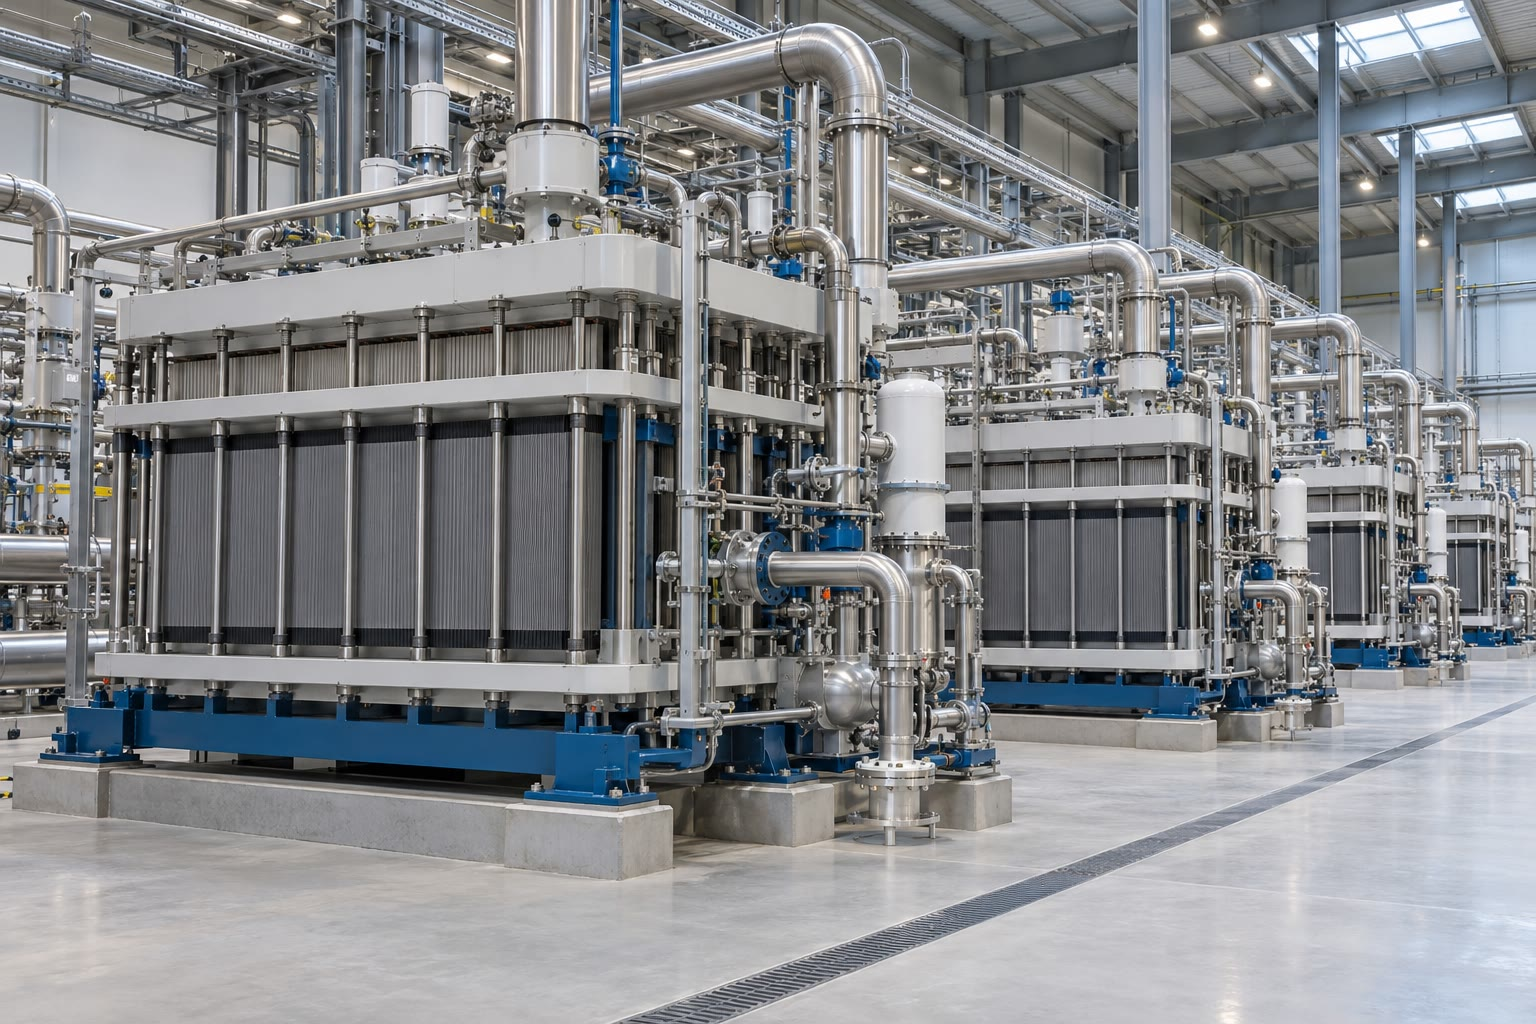
\includegraphics[width=0.48\linewidth]{images/book1/ai/g12-electrolyser-hall.jpg}

{\small 电解车间：水被分解为氢气和
氧气。}
\end{omfigure}

\section{练习}

\begin{exercise}[$\star$]\label{exo:g12:cells-and-electrolysis:1}
在丹尼尔电池中，哪一个电极是阳极？哪一个是阴极？写出
每个电极上的半反应式。
\end{exercise}

\begin{exercise}[$\star$]\label{exo:g12:cells-and-electrolysis:2}
通以 \qty{0.20}{A} 的电流，持续 \qty{30}{min}。计算所通过的电荷量
及电子的物质的量。
\end{exercise}

\begin{exercise}[$\star$]\label{exo:g12:cells-and-electrolysis:3}
盐桥起什么作用？若将其移去，会发生什么？
\end{exercise}

\begin{exercise}[$\star$]\label{exo:g12:cells-and-electrolysis:4}
将电量 \qty{2.5}{A.h} 换算为库仑。
\end{exercise}

\begin{exercise}[$\star$]\label{exo:g12:cells-and-electrolysis:5}
电解过程中，该反应是否自发进行？提供
能量的是什么？
\end{exercise}

\begin{exercise}[$\star\star$]\label{exo:g12:cells-and-electrolysis:6}
一个原电池由浸在硝酸银溶液中的银电极和
浸在硫酸铜溶液中的铜电极组成。电压表显示电子
由铜电极流出。写出半反应式，指出阳极和阴极，
并写出总反应。
\end{exercise}

\begin{exercise}[$\star\star$]\label{exo:g12:cells-and-electrolysis:7}
一枚手表电池持续三年输出 \qty{10}{\micro A} 的电流。
其电量为多少 \si{mA.h}？
\end{exercise}

\begin{exercise}[$\star\star$]\label{exo:g12:cells-and-electrolysis:8}
用 \qty{0.50}{A} 的电流为一把勺子镀银，持续
\qty{40}{min}，\ce{Ag+ + e- -> Ag}。析出银的质量为多少？
\end{exercise}

\begin{exercise}[$\star\star$]\label{exo:g12:cells-and-electrolysis:9}
在丹尼尔电池的示意图上，标出导线中电流的方向，
并标出盐桥中 \ce{K+} 与 \ce{NO3-} 离子
的移动方向。
\end{exercise}

\begin{exercise}[$\star\star$]\label{exo:g12:cells-and-electrolysis:10}
比较原电池与电解池：阳极的符号、反应的
方向、能量的转化。
\end{exercise}

\begin{exercise}[$\star\star$]\label{exo:g12:cells-and-electrolysis:11}
电解水时，收集到 \qty{24}{mL} 氢气。
同时可收集到多少体积的氧气？为什么？
\end{exercise}

\begin{exercise}[$\star\star\star$]\label{exo:g12:cells-and-electrolysis:12}
一个丹尼尔电池中含有 \qty{5.0}{g} 锌和 \qty{100}{mL}
浓度为 \qty{0.50}{mol/L} 的硫酸铜溶液。哪种反应物会先耗尽？该电池的
电量是多少？它能以 \qty{50}{mA} 的电流持续供电多久？
\end{exercise}

\begin{exercise}[$\star\star\star$]\label{exo:g12:cells-and-electrolysis:13}
一节电压为 \qty{1.5}{V} 的电池，输出 \qty{2.0}{A.h} 的电量。计算它
储存的能量（$E = Q U$），分别用焦耳和瓦时表示。
\end{exercise}

\begin{exercise}[$\star\star\star$]\label{exo:g12:cells-and-electrolysis:14}
用 \qty{2.0}{A} 的电流电解水 \qty{1.0}{h}。计算所生成
的氢气与氧气的物质的量，再算出在 \qty{20}{\celsius} 下（$V_m = \qty{24.1}{L/mol}$）
的体积。
\end{exercise}

\begin{exercise}[$\star\star\star$]\label{exo:g12:cells-and-electrolysis:15}
在粗铜精炼中，阳极失去 \qty{3.00}{kg} 物质，阴极
获得 \qty{2.84}{kg} 铜。粗阳极中铜的质量分数是多少？
假设阳极上只有铜被氧化，
杂质直接脱落。
\end{exercise}

\section{问题：手机电池}

\begin{problem}[{周末问题——一块 \qty{4000}{mA.h} 手机电池的电极之间
往返穿梭的锂有多少质量？}]
\label{pb:g12:cells-and-electrolysis:1}
% ledger: const:F, const:NA, aw:Li, dch:CH4, aw:C, aw:H
一块手机电池上标有“\qty{3.7}{V}，\qty{4000}{mA.h}”。按照简化的
模型，放电时，储存在石墨电极中的每个锂原子
失去一个电子，以锂离子的形式离开，
\ce{Li -> Li+ + e-}；离子穿过电解质，
被金属氧化物电极接收，该电极同时得到一个电子。

\medskip
\noindent\textbf{第一部分——电池。}
\begin{enumerate}
  \item 放电时，石墨电极是阳极还是
        阴极？为什么？
  \item 哪一个是负极接线柱？
  \item 电子在手机中沿哪个方向移动？
        电池内部的锂离子呢？
  \item 为什么这种电池属于蓄电池？
\end{enumerate}

\medskip
\noindent\textbf{第二部分——电量。}
\begin{enumerate}[resume]
  \item 将 \qty{4000}{mA.h} 换算为安时，再换算为库仑。
  \item 计算这些电量所对应的电子的物质的量。
  \item 这些电子有多少个？
  \item 手机平均工作电流为 \qty{0.25}{A}。充满电的
        电池能使用多长时间？
  \item 屏幕显示电量为 20 \%。剩余的电量为多少库仑？
\end{enumerate}

\medskip
\noindent\textbf{第三部分——能量。}
\begin{enumerate}[resume]
  \item 计算所储存的能量 $E = Q U$（以焦耳为单位）。
  \item 将其换算为瓦时。
  \item 将其与燃烧 \qty{1}{g} 甲烷所释放的能量进行比较，
        （\qty{55.7}{kJ}）。
  \item \qty{1}{kW.h} 的电能，若无任何能量损失，
        可供多少次完整充电？
\end{enumerate}

\medskip
\noindent\textbf{第四部分——再充电。}
\begin{enumerate}[resume]
  \item 充电时，石墨电极上发生哪个反应？
        该反应属于氧化还是还原？
  \item 为什么充电属于电解过程？
  \item 充电器输出 \qty{2.0}{A} 的电流。充满电
        至少需要多长时间？
  \item 一次完整充电过程中，穿过电解质的锂离子
        的物质的量是多少？
  \item 计算它们的质量。
  \item 给出最终结果：一次完整充电中，在两电极
        之间往返穿梭的锂的质量是多少？
\end{enumerate}
\end{problem}
